% ============================================================
%  COUVERTURE — Mazava Maths · Terminale S
%  Système éducatif malagasy | Série S
%  © 2025 Mamiarilala
% ============================================================
\begin{titlepage}
	
	\newgeometry{
		top    = 0cm,
		bottom = 0cm,
		left   = 0cm,
		right  = 0cm,
	}
	
	% ── Bandeau supérieur noir ───────────────────────────────────
	\noindent\colorbox{black}{%
		\begin{minipage}[t][\dimexpr0.30\textheight+2cm\relax][t]{\paperwidth}%
			\color{white}%
			\vspace{2.0cm}%
			\begin{center}
				{\fontsize{30}{34}\selectfont\bfseries Mazava Maths}\\[0.5cm]
				{\large\MakeUppercase{Terminale \quad—\quad Série S}}\\[0.4cm]
				{\small\color{white!60!black}
					Système éducatif malagasy}\\[0.3cm]
				{\small\color{white!40!black}\rule{4.5cm}{0.3pt}}
			\end{center}
			\vfill
		\end{minipage}%
	}
	
	\vspace{0.65cm}
	
	% ── Filet double ────────────────────────────────────────────
	\noindent\hspace{1.5cm}%
	\begin{minipage}{\dimexpr\paperwidth-3cm\relax}
		\rule{\linewidth}{1.2pt}\\[2pt]
		\rule{\linewidth}{0.3pt}
	\end{minipage}
	
	\vspace{0.65cm}
	
	% ── Sous-titre descriptif ────────────────────────────────────
	\begin{center}
		{\small\MakeUppercase{%
				\bfseries Cours\quad·\quad Exercices\quad·\quad Sujets-types corrigés}}
	\end{center}
	
	\vspace{0.8cm}
	
	% ── Zone graphique TikZ ──────────────────────────────────────
	\begin{center}
		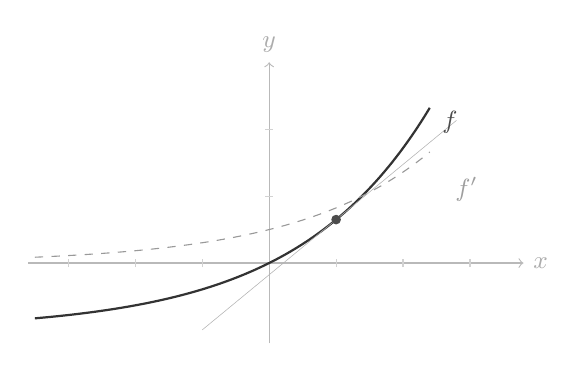
\begin{tikzpicture}[scale=0.85]
			
			% Axes
			\draw[->, thin, gray!55]
			(-3.6,0) -- (3.8,0)
			node[right, font=\small\itshape, gray!65] {$x$};
			\draw[->, thin, gray!55]
			(0,-1.2) -- (0,3.0)
			node[above, font=\small\itshape, gray!65] {$y$};
			
			% Graduations
			\foreach \x in {-3,-2,-1,1,2,3} {
				\draw[gray!35, thin] (\x,-0.06) -- (\x,0.06);
			}
			\foreach \y in {1,2} {
				\draw[gray!35, thin] (-0.06,\y) -- (0.06,\y);
			}
			
			% Courbe f(x) = e^(x/2) - 1
			\draw[black!80, thick, smooth, domain=-3.5:2.4, samples=80]
			plot (\x, {exp(\x/2)-1});
			
			% Dérivée f'(x) = 0.5*e^(x/2)  (pointillés fins)
			\draw[black!40, thin, dashed, smooth, domain=-3.5:2.4, samples=80]
			plot (\x, {0.5*exp(\x/2)});
			
			% Tangente en x=1
			\draw[black!30, very thin, domain=-1.0:2.8]
			plot (\x, {0.824*(\x-1)+0.649});
			
			% Point de tangence
			\filldraw[black!70] (1, 0.649) circle (1.8pt);
			
			% Étiquettes
			\node[font=\small\itshape, black!70] at (2.7, 2.1) {$f$};
			\node[font=\small\itshape, black!38] at (2.95,1.1) {$f'$};
			
		\end{tikzpicture}
	\end{center}
	
	\vfill
	
	% ── Filet double avant pied ──────────────────────────────────
	\noindent\hspace{1.5cm}%
	\begin{minipage}{\dimexpr\paperwidth-3cm\relax}
		\rule{\linewidth}{0.3pt}\\[2pt]
		\rule{\linewidth}{1.2pt}
	\end{minipage}
	
	\vspace{0.5cm}
	
	% ── Pied de page ────────────────────────────────────────────
%	\begin{center}
%		{\normalsize\bfseries Mamiarilala}\\[0.25cm]
%		{\small Année scolaire 2026\,–\,2027}\\[0.25cm]
%		{\footnotesize\color{black!45}
%			\textcopyright\ 2025 Mamiarilala\quad—\quad Tous droits réservés}
%	\end{center}
	
	\vspace{0.6cm}
	
	\restoregeometry
\end{titlepage}

% ── Page de copyright (verso couverture) ─────────────────────
\thispagestyle{empty}
\vspace*{\fill}
\begin{flushleft}
	\small
	\textbf{Mazava Maths — Terminale S}\\[0.4cm]
	\textcopyright\ 2025 Mamiarilala\\[0.2cm]
	Tous droits réservés.\\
	Toute reproduction, même partielle, est interdite\\
	sans autorisation écrite de l'auteur.\\[0.4cm]
	\textit{Conforme au programme officiel}\\
	\textit{du système éducatif malagasy — Série S}\\-X-XXXXXX-XX-X
%	Dépôt légal : 2025\\
%	Imprimé à Madagascar
\end{flushleft}
\newpage